\documentclass{article}
\usepackage[utf8]{inputenc}
\usepackage[T1]{fontenc}
\usepackage{geometry}
\geometry{left=2.5cm,right=2.5cm,top=2.5cm,bottom=2.5cm}
\usepackage{graphicx}
\usepackage{float}
\usepackage{amsmath}
\usepackage{amssymb}
\usepackage{cite}
\usepackage{hyperref}
\usepackage{listings}
\usepackage{xcolor}
\usepackage{booktabs}
\usepackage{caption}
\usepackage{subcaption}
\usepackage{algorithm}
\usepackage{algpseudocode}
\usepackage{tikz}
\usepackage{pgfplots}
\pgfplotsset{compat=1.16}
\usetikzlibrary{shapes,arrows,positioning,fit,backgrounds,matrix,calc}

\definecolor{bluebox}{RGB}{230,240,255}
\definecolor{greenbox}{RGB}{230,255,230}
\definecolor{redbox}{RGB}{255,230,230}
\definecolor{orangebox}{RGB}{255,245,220}

\lstset{
    basicstyle=\ttfamily\small,
    breaklines=true,
    frame=single,
    backgroundcolor=\color{gray!10},
    keywordstyle=\color{blue},
    commentstyle=\color{green!60!black},
    stringstyle=\color{red}
}

\title{A GDPR Compliance Warning Framework Based on Android Permission Auditing: Design, Implementation and Adversarial Evaluation}
\author{Zhiheng Zhang}
\date{July 2026}

\begin{document}

\maketitle
\newpage
\tableofcontents
\newpage

% Chapter 1 Revision 04
% Chapter 1 Revision 03
% ==================== Chapter 1: Introduction (Revision 02) ====================
\newpage
\begin{abstract}
Mobile applications routinely access location, microphone, and contact data, yet platform permission interfaces provide limited support for interpreting whether repeated access is proportionate to a declared purpose. This thesis presents and evaluates a prototype GDPR compliance-warning application that translates permission-access counts into explainable risk findings. The implemented React Native/TypeScript prototype contains a modular compliance engine, explicit rule metadata for three sensitive permission categories, a deterministic threshold calculation, local finding persistence, a violation simulator, and an Android user interface for running and reviewing audits.

Evaluation was performed at both the logical and packaged-application layers. An independent-oracle Monte Carlo test and a boundary-stratified test produced 7,000 zero-error observations for the implemented daily-count rule, with a descriptive 95\% Wilson accuracy lower bound of 99.945\%. A release-APK endurance sequence added 1,500 zero-error integration observations, completed without a captured crash or application-not-responding event, and recorded a peak proportional set size of 115.16~MB. These results validate implementation consistency within the specified rule domain.

A second adversarial campaign exposed limits that conventional accuracy did not reveal. Short-term burst and cross-window split attacks each bypassed the detector in all tested scenarios; all 40,000 invalid time windows were accepted; and 83.776\% of 250,000 combined malformed inputs were silently classified as normal. The study therefore distinguishes rule correctness from threat-model completeness. It concludes that the prototype is a reproducible compliance-warning demonstrator, while production deployment requires fail-closed runtime validation, multi-scale temporal features, privileged or system-mediated Android data acquisition, physical-device endurance testing, and legal review of the warning criteria.
\end{abstract}

\section{Introduction}

\subsection{Background and Motivation}

The General Data Protection Regulation (GDPR) requires personal data to be processed lawfully, transparently, and in a manner limited to what is necessary for the stated purpose. On Android, runtime permission controls make access decisions visible to users, but a grant or denial does not by itself explain whether the frequency of subsequent access is proportionate. A navigation application and a calculator may both request location permission, yet identical access counts can carry very different contextual meanings. Permission frequency is therefore a useful warning signal, but it is not, on its own, a legal determination.

This thesis investigates whether a small, explainable rule engine can turn structured permission-audit observations into reproducible compliance warnings. The work focuses on three sensitive categories represented in the prototype: LOCATION, MICROPHONE, and CONTACTS. For each category, the engine records a baseline, a deviation multiplier, a GDPR mapping, and a plain-language rationale. An observation becomes active when its access count strictly exceeds the calculated threshold. The approach favours transparency: every finding exposes the rule, threshold, excess count, risk level, and regulatory rationale that produced it.

The research is motivated by a practical gap between platform transparency and compliance interpretation. Native privacy dashboards provide useful histories, but users must still interpret whether a pattern is excessive, whether an abnormal record is trustworthy, and whether repeated notifications deserve attention. Conversely, opaque anomaly models may produce a score without an auditable reason. A deterministic prototype provides a controlled setting in which the relationship between an observation and a warning can be examined directly.

\subsection{Problem Statement}

The central problem is not simply to maximise classification accuracy. It is to establish what a warning means, which inputs it trusts, and which behaviours its model can observe. Three related challenges follow.

\begin{enumerate}
    \item \textbf{Explainable operationalisation.} GDPR principles are contextual legal standards. A software prototype must not claim that a frequency threshold proves illegality. It can, however, identify a pattern that warrants review and show the rule used to reach that conclusion.
    \item \textbf{Reliable implementation.} The same structured observation must produce the same result across random, boundary, and repeated APK execution. An external test oracle is required to avoid validating the implementation against itself.
    \item \textbf{Adversarial completeness.} High accuracy over valid count inputs does not establish resistance to burst timing, cross-window splitting, forged timestamps, type confusion, or malformed permission identifiers. These dimensions require separate oracles and metrics.
\end{enumerate}

This distinction is especially important for a compliance tool. A false assurance can be more harmful than an explicit rejection because it may enter an audit trail as an apparently valid normal result. The framework is therefore evaluated for both incorrect classifications and unsafe acceptance.

\subsection{Research Questions}

The study addresses the following research questions:

\begin{enumerate}
    \item Can a modular, explainable engine implement permission-specific aggregate-count warning rules consistently across random and boundary inputs?
    \item Does the packaged Android application preserve this correctness and remain operational during accelerated repeated execution?
    \item Which previously unmodelled temporal and runtime-input attacks can bypass or destabilise the current prototype?
    \item What implementation and validation work is required before the prototype can support broader operational claims?
\end{enumerate}

\subsection{Objectives and Contributions}

The first objective is to produce an auditable prototype rather than an opaque classifier. The TypeScript \texttt{GDPRComplianceEngine} implements the \texttt{IComplianceEngine} interface and uses an explicit rule table. The current thresholds are calculated as the ceiling of a fixed baseline multiplied by 1.5: 36 for LOCATION, 12 for MICROPHONE, and 6 for CONTACTS. Findings retain the permission, package identifier, threshold, excess count, risk level, detection time, GDPR article mapping, and rationale.

The second objective is to connect this logic to a usable Android demonstrator. The React Native application provides experiment, privacy, history, scoring, and settings views. Synthetic configurations are converted into audit observations, evaluated locally, and persisted with AsyncStorage. The repository also contains a native-bridge boundary for future Android acquisition and scheduling functions. Those optional native functions are not treated as validated production capabilities in this thesis.

The third objective is methodological. The evaluation separates independent-oracle logical tests, release-APK integration tests, and adversarial tests. The contribution is not merely a large execution count, but an evidence structure that prevents a correct implementation of a narrow rule from being presented as complete attack detection.

The principal contributions are:

\begin{itemize}
    \item an explainable and modular compliance-warning rule engine for three sensitive permission categories;
    \item a locally operated Android demonstrator with reproducible simulation and finding persistence;
    \item a progressive validation protocol combining independent random sampling, threshold-boundary stratification, APK endurance, and Android event fuzzing;
    \item a second adversarial protocol that quantifies temporal bypass, invalid-window acceptance, runtime type confusion, permission-key mutation, and combined malformed inputs; and
    \item an evidence-based set of priorities for fail-closed validation, temporal modelling, UI regression, and future native Android integration.
\end{itemize}

\subsection{Scope}

The implemented and evaluated scope is deliberately bounded. The engine evaluates structured observations supplied by the simulator or application workflow. The study does not demonstrate unrestricted collection of other applications' permission history on a stock physical device, does not establish 24- or 72-hour WorkManager reliability, and does not measure battery drain. It also does not determine GDPR liability. The output is a warning that supports review, not a binding legal conclusion.

This boundary improves rather than weakens the research claim. It permits the tested logic, APK behaviour, observed vulnerabilities, and untested production assumptions to be stated separately. The resulting account is reproducible and avoids attributing native Android capabilities to code paths that were not exercised.

\subsection{Thesis Structure}

Chapter 2 reviews GDPR principles, privacy-warning design, Android auditing constraints, and security-testing methods. Chapter 3 derives the requirements and presents the architecture of the implemented prototype, including explicit trust boundaries. Chapter 4 explains the TypeScript rule engine, simulator, local repository, bridge boundary, and user-interface integration. Chapter 5 reports both iterative test campaigns and their statistical interpretation. Chapter 6 discusses trade-offs, validity, legal and platform limitations, and repair priorities. Chapter 7 answers the research questions, summarises the supported contributions, and defines the work required for a production-oriented system.

\subsection{Revised Research Emphasis}

The final iteration places GDPR accountability and compliance evidence at the centre of the research. Permission-frequency and temporal signals are treated as technical observations that may trigger review. They are not substitutes for purpose, lawful basis, controller identity, retention limits, special-category conditions, or human legal assessment. The principal research question is therefore whether an Android warning framework can preserve a traceable chain from technical observation to cautious compliance review without overstating what the evidence proves.

Human-computer interaction and psychological theory form a secondary question: whether uncertainty, evidence gaps, and recommended actions can be communicated in a manner that supports calibrated trust and avoids notification fatigue. This ordering prevents usability metrics from becoming proxies for compliance and prevents legally incomplete evidence from being made persuasive merely through interface design.

\subsection{Integrated Research Position}

The final prototype is evaluated as an accountability support system rather than an automated legal adjudicator. Its contribution combines permission-access signals, explicit evidence gaps, calibrated warnings, human review and measurable interaction cost. This preserves the compliance emphasis of the original framework while retaining the later HCI and performance perspectives. GDPR Articles 5 and 25 motivate accountability and data protection by design, but neither makes an access-frequency threshold a legal verdict \cite{eurlex2016,edpb2019}.

Accordingly, the research question is operationalised at three levels: whether controlled technical misuse is detected; whether the interface communicates uncertainty and action without deceptive pressure; and whether the Android implementation remains usable and stable under device and event-load variation. Performance and HCI evidence qualify the claim rather than displacing the legal analysis.


% Chapter 2 Revision 05
% Chapter 2 Revision 04
% ==================== Chapter 2: Literature Review (Revision 03) ====================
\newpage
\section{Literature Review and State of the Art}

\subsection{From GDPR Principles to Technical Warning Signals}

Article 5 of the GDPR establishes lawfulness, fairness, transparency, purpose limitation, data minimisation, accuracy, storage limitation, integrity, confidentiality, and accountability \cite{1}. Article 5(1)(c) requires personal data to be adequate, relevant, and limited to what is necessary. Article 25 further requires data protection by design and by default. These provisions motivate technical mechanisms that make data processing observable, but they do not define a universal numeric limit for permission access.

This distinction determines the role of the proposed framework. A high access count may be legitimate for navigation and disproportionate for a calculator. A threshold crossing is therefore an auditable warning signal rather than proof of a GDPR infringement. Purpose, lawful basis, user expectations, foreground context, data destination, and safeguards remain relevant to any legal assessment. The prototype operationalises only one observable component: whether a structured permission count exceeds an explicit, permission-specific rule.

Article 7 concerns the conditions for consent and withdrawal, while Article 9 imposes additional conditions on special-category data. Location, microphone, and contact information are not automatically special-category data in every context, although they may reveal health, biometric, religious, political, or other protected information. The engine's GDPR mappings are consequently explanatory prompts. They identify provisions that may require review and do not replace a controller's legal analysis.

\subsection{Transparency, Cognitive Load, and Warning Design}

Privacy notices impose a substantial verification burden on users. Long policies and frequent prompts encourage heuristic decision-making, while repeated low-value warnings can create habituation and privacy fatigue \cite{12,13,27}. Cognitive Load Theory suggests that information should be structured so that users can identify the reason for an intervention without processing unnecessary detail \cite{27}. Trust in automation likewise depends on calibrated rather than unconditional reliance \cite{34}.

These findings support three interface principles used by the prototype. First, a finding should expose its threshold, observed count, risk level, and rationale. Second, unchanged findings should not repeatedly demand attention. Third, severity should be interpretable and should not imply legal certainty. The local repository therefore records whether a finding changed and whether notification would be justified by a state transition or risk escalation.

The evaluation in this thesis does not include a user study. Claims that the interface reduces cognitive load or improves privacy decisions remain design hypotheses. A longitudinal study using behavioural measures and instruments such as NASA-TLX would be required to validate those effects \cite{6}.

\subsection{Android Permission Transparency and Acquisition Constraints}

Android has progressively expanded runtime permission controls and system privacy interfaces. The Privacy Dashboard introduced a system-managed history for selected sensitive permissions, providing users with temporal visibility. However, access to app-operation history by a third-party application is constrained by Android version, privileges, attribution, and vendor implementation. Public presence of an \texttt{AppOpsManager} method does not imply that an ordinary sandboxed application can retrieve unrestricted histories for every other package.

This constraint divides a complete system into two parts. The decision layer can be implemented and tested using structured \texttt{PermissionAudit} observations. The acquisition layer requires an authorised source, such as system integration, device-owner deployment, user-mediated export, or another platform-supported mechanism. The current repository validates the former and exposes a React Native native-module boundary for the latter; it does not claim that unrestricted cross-application acquisition was demonstrated on a stock physical device.

Static-analysis systems such as FlowDroid and dynamic taint-tracking systems address different questions. They seek code paths or data flows from sensitive sources to sinks, often at greater deployment and computational cost. VPN-based monitoring observes network traffic but cannot directly observe local permission use and introduces its own trust boundary. Native dashboards are low-overhead and authoritative but do not provide the custom rule evaluation developed here. The proposed prototype therefore occupies a narrower position: explainable evaluation of supplied permission-frequency observations.

\subsection{Rule-Based and Statistical Detection}

Rule-based systems are attractive for compliance warnings because their outputs can be traced to an explicit condition. They also expose their limitations. A fixed threshold ignores temporal concentration and application purpose, while a learned anomaly model can be difficult to explain and may drift as behaviour changes. Hybrid systems may combine population priors, per-user history, and contextual features, but those additions require empirical data and independent validation.

The implemented prototype uses fixed expert-configured baselines multiplied by 1.5. It does not compute a rolling mean, standard deviation, or three-sigma threshold, and it does not contain a validated population study of the top 50 applications. Those mechanisms remain possible extensions, not evaluated features. This factual boundary is essential because a claimed adaptive model cannot be supported by experiments that exercise a deterministic fixed rule.

The current rule is intentionally simple:

\begin{equation}
T_p=\left\lceil 1.5B_p \right\rceil,\qquad
A(x,p)=\mathbb{I}[x>T_p],
\end{equation}

where $B_p$ is the configured baseline for permission $p$, $T_p$ is the threshold, $x$ is the supplied access count, and $A$ is the active-warning decision. Simplicity makes exhaustive boundary reasoning possible, but it also makes temporal bypass predictable unless time-derived features are added.

\subsection{Randomised, Boundary, and Adversarial Validation}

Randomised testing explores a larger input space than a small hand-written suite. Its value depends on the oracle and distribution. If the expected result is produced by the same helper used by the system under test, perfect agreement may merely demonstrate shared logic. The evaluation therefore introduces an external oracle for the main Monte Carlo round and separately concentrates samples at $T_p-2$ through $T_p+2$.

Boundary testing is necessary because random uniform inputs may rarely land close to a threshold. Adversarial testing asks a different question: what happens when assumptions are violated? Fuzzing permission keys, numeric types, and time windows tests the runtime trust boundary; burst and split-window samples test omissions in the decision model. These cases cannot all be placed in a conventional confusion matrix, because they use different threat definitions and expected failure policies.

Confidence intervals are also required for honest interpretation. An observed accuracy of 100\% is a point estimate. Wilson intervals and the rule of three express the uncertainty remaining after zero observed errors. Repeated deterministic mutations are useful for stress and reproducibility, but repetitions of the same mutation class should not be described as independent population samples.

\subsection{Research Gap}

Prior approaches typically emphasise one of four goals: platform transparency, static disclosure analysis, data-flow detection, or user notification. The research gap addressed here is a reproducible connection between an explainable permission-frequency rule, a usable Android demonstrator, and an evaluation that explicitly separates correctness from adversarial coverage.

The contribution is accordingly methodological as well as technical. The prototype demonstrates how a compliance-warning decision can be exposed and tested. The negative adversarial results demonstrate why a narrow rule must not be generalised into a claim of complete GDPR compliance detection. Chapters 3 and 4 translate this position into explicit architecture and implementation boundaries, and Chapter 5 evaluates both the supported rule and its uncovered attack surface.

\subsection{GDPR Accountability as the Primary Analytical Lens}

The revised framework places GDPR compliance reasoning ahead of interface optimisation. Article 5 supplies the controlling principles: lawfulness, fairness and transparency; purpose limitation; data minimisation; storage limitation; security; and accountability. Article 6 requires an identified lawful basis, while Article 9 adds a separate condition when the processing concerns special-category data. Article 25 requires data protection to be embedded by design and by default and treated as a continuing duty rather than a one-time interface choice.

Permission frequency is therefore evidence, not a compliance conclusion. A defensible assessment also needs a specified purpose, controller identity, lawful basis, retention period, processing context, and, where applicable, an Article 9 condition. The prototype now represents these elements explicitly and classifies missing documentation as insufficient evidence. This implements accountability more faithfully than converting every threshold crossing into a claimed infringement.

Human-computer interaction remains relevant but subordinate. Cognitive load, trust calibration, and notification fatigue determine whether a legally cautious warning is understood. They do not determine whether processing is lawful. The interface contribution is consequently limited to progressive disclosure, neutral wording, explicit uncertainty, and notification priority proportional to the evidence.

The design follows the European Data Protection Board's position that data protection by design and by default is continuous and that privacy-protective defaults must be built into systems and reviewed as risks change. The framework operationalises this position through fail-closed inputs, evidence-gap reporting, local processing, and an explicit prohibition on presenting automated output as a legal adjudication.

\subsection{Compliance-Centred Universal Interaction Design}

The redesign connects data protection by design with established usability and accessibility requirements. The EDPB requires safeguards to be embedded throughout processing and warns against interfaces that overload, obstruct or steer data subjects \cite{edpb2019,edpb2022}. WCAG 2.2 requires that colour is not the sole carrier of meaning and provides minimum contrast and target-size criteria \cite{wcag22}. Android guidance additionally recommends touch targets of at least 48~dp and meaningful accessibility descriptions \cite{androidaccess}.

These sources support four interface decisions: textual status markers supplement colour; primary decisions use 48--52~dp targets; a persistent caveat separates technical warning from legal verdict; and progressive disclosure presents status and recommended action before detailed telemetry. The design aims at effectiveness, efficiency and satisfaction in the ISO 9241-11 sense \cite{iso924111}, while recognising that conformance-oriented inspection cannot replace participant testing.


% Chapter 3 Revision 06
% Chapter 3 Revision 05
% ==================== Chapter 3: Requirements and Architecture (Revision 04) ====================
\newpage
\section{System Requirements and Overall Design}

\subsection{System Boundary}

The system is a local compliance-warning demonstrator. Its validated input is a structured \texttt{PermissionAudit} containing a package name, one of three supported permission categories, an access count, and an audit-window start and end. Its validated output is an explainable \texttt{ComplianceFinding}. The framework does not intercept calls, block data transfer, determine legal liability, or prove that consent withdrawal has been enforced by another application.

The Android application is implemented with React Native, Expo, and TypeScript. It contains an optional native-module boundary named \texttt{PrivacyInspector}, but the evaluated build does not establish unrestricted acquisition of other applications' AppOps history. Acquisition and decision are therefore separate trust domains:

\begin{itemize}
    \item the \textbf{acquisition domain} is responsible for producing authentic, well-formed observations under an Android-supported authority model;
    \item the \textbf{decision domain} evaluates those observations using transparent rules; and
    \item the \textbf{presentation domain} stores and displays findings without upgrading a warning into a legal conclusion.
\end{itemize}

\subsection{Functional Requirements}

The implemented prototype must:

\begin{enumerate}
    \item evaluate LOCATION, MICROPHONE, and CONTACTS observations through a common engine interface;
    \item expose the threshold, excess count, risk level, GDPR mapping, rationale, and detection time;
    \item generate reproducible benign and violating simulation cases;
    \item persist the latest finding for each package-permission pair locally;
    \item identify whether a finding changed or escalated;
    \item display experiment and privacy results in the Android application; and
    \item permit release-build testing through adb-driven interaction and evidence capture.
\end{enumerate}

Security requirements derived from the adversarial model are stricter than the initial implementation. Permission values must belong to an explicit whitelist. Counts must be finite, non-negative integers. Window timestamps must be finite integers with a valid ordering and bounded duration. Invalid input must produce a structured rejection and an audit record. These requirements are included in the final architecture even though Chapter 5 shows that the current engine does not yet satisfy them.

\subsection{Non-Functional Requirements}

The principal non-functional requirements are explainability, reproducibility, local operation, and bounded resource use. A fixed seed must reproduce logical test sequences. Findings must be understandable without inspecting source code. Personal audit data should remain on the device unless the user deliberately exports it. The release application should remain responsive and below the provisional 150~MB PSS target during accelerated evaluation.

Battery consumption, multi-day scheduling, and manufacturer-specific background behaviour are not accepted as satisfied requirements because they were not measured. They are validation requirements for a future native acquisition layer.

\subsection{Architecture}

The architecture contains five cooperating components.

\begin{enumerate}
    \item \textbf{Compliance engine.} \texttt{GDPRComplianceEngine} implements \texttt{IComplianceEngine} and evaluates one structured audit at a time.
    \item \textbf{Rule configuration.} \texttt{GDPR\_RULES} stores the baseline, deviation multiplier, GDPR mapping, and rationale for each supported permission.
    \item \textbf{Simulation and evaluation.} \texttt{ViolationSimulator} generates configurations and converts them to audits. Evaluation code records confusion-matrix outcomes.
    \item \textbf{Finding repository.} \texttt{ViolationRepository} uses AsyncStorage and determines whether a finding is new, changed, or escalated.
    \item \textbf{Application and bridge boundary.} React Native screens invoke the TypeScript services. \texttt{PrivacyBridge} optionally delegates acquisition, scheduling, and dispatch functions to a native \texttt{PrivacyInspector} module when one is present.
\end{enumerate}

\begin{figure}[H]
\centering
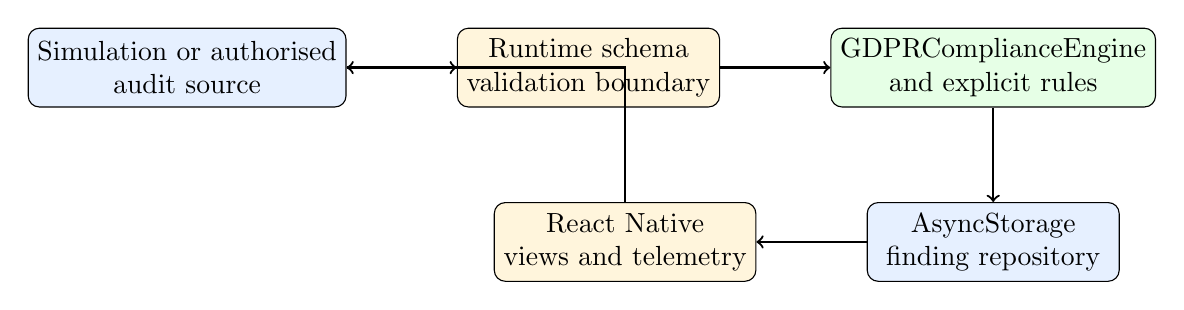
\begin{tikzpicture}[
node distance=1.2cm and 1.4cm,
box/.style={draw, rounded corners, align=center, minimum width=3.2cm, minimum height=1cm},
arrow/.style={->, thick}
]
\node[box, fill=bluebox] (source) {Simulation or authorised\\audit source};
\node[box, fill=orangebox, right=of source] (validation) {Runtime schema\\validation boundary};
\node[box, fill=greenbox, right=of validation] (engine) {GDPRComplianceEngine\\and explicit rules};
\node[box, fill=bluebox, below=of engine] (repo) {AsyncStorage\\finding repository};
\node[box, fill=orangebox, left=of repo] (ui) {React Native\\views and telemetry};
\draw[arrow] (source) -- (validation);
\draw[arrow] (validation) -- (engine);
\draw[arrow] (engine) -- (repo);
\draw[arrow] (repo) -- (ui);
\draw[arrow] (ui) |- (source);
\end{tikzpicture}
\caption{Prototype architecture and the required input-validation boundary}
\label{fig:final-architecture}
\end{figure}

The validation boundary is shown explicitly because it is the highest-priority missing control identified by testing. Its architectural placement ensures that no malformed value reaches threshold lookup or arithmetic.

\subsection{Decision Model}

For each permission $p$, the engine calculates

\begin{equation}
T_p=\max(1,\lceil B_pM_p\rceil),
\end{equation}

where $B_p$ is the configured baseline and $M_p=1.5$. The implemented baselines are 24, 8, and 4, yielding thresholds of 36, 12, and 6. The excess and ratio are

\begin{equation}
E=\max(0,x-T_p),\qquad R=E/T_p.
\end{equation}

A finding is active when $E>0$. Active findings are mapped to MEDIUM, HIGH, or CRITICAL according to the excess ratio; inactive findings are LOW. These severity labels prioritise review and do not state the severity of a legally adjudicated GDPR violation.

\subsection{Temporal Model and Known Coverage Gap}

The input structure contains trigger times and window fields, but the current decision uses only the aggregate count. Consequently, uniform and burst distributions with the same count receive the same verdict, and adjacent windows do not share cumulative state. The final design therefore specifies a later temporal layer containing peak rate, minute/hour/day windows, and decaying cross-window state. This layer is a repair requirement, not an implemented result.

\subsection{Validation Architecture}

Validation proceeds in layers:

\begin{enumerate}
    \item deterministic checks for rule and boundary semantics;
    \item independent-oracle Monte Carlo sampling;
    \item release-APK workflow and repeated endurance evaluation;
    \item adversarial temporal, window, type, and key mutation;
    \item Android random-event testing and replay; and
    \item future physical-device, native-source, and long-duration testing.
\end{enumerate}

Each layer has its own oracle. Classification metrics are used only when positive and negative labels are meaningful. Rejection rate, silent-normal rate, non-finite-output rate, bypass rate, process survival, memory, and frame evidence are reported for adversarial and APK stages.

\subsection{Summary}

The final architecture aligns claims with executable artefacts. It treats native permission acquisition as a separate, privilege-sensitive component; defines the TypeScript rule engine as the evaluated core; makes runtime validation an explicit missing security boundary; and preserves a clear path from a generated observation to an explainable stored finding.

\subsection{Compliance Evidence and Human Review Architecture}

The final requirements distinguish three layers. The technical layer detects aggregate, burst, and cross-window signals. The compliance layer evaluates whether the audit includes purpose, Article 6 lawful basis, controller identity, retention period, and any required Article 9 condition. The presentation layer communicates the result without collapsing uncertainty into a binary legal label.

Four compliance states are defined: \texttt{INSUFFICIENT\_EVIDENCE}, \texttt{REVIEW\_REQUIRED}, \texttt{LIKELY\_NON\_COMPLIANT}, and \texttt{NO\_TECHNICAL\_CONCERN}. The last state is deliberately narrower than ``compliant''. It only states that the supplied technical observation contains no modelled anomaly and that the declared context is complete enough for this limited check. Final legal responsibility remains with the controller and human reviewer.

The architecture treats evidence completeness as a first-class requirement. Processing based on consent is escalated when consent is recorded as withdrawn and access continues. Special-category processing requires an Article 9 condition in addition to its Article 6 basis. Invalid context values are rejected at the same trust boundary as invalid counts and timestamps.

The secondary HCI requirement is calibrated communication. No-concern observations are silent; evidence gaps and ordinary anomalies receive standard review prompts; likely non-compliance or critical technical risk is urgent. Every message includes a short reason and a recommended human action, preventing the warning system from substituting interface confidence for legal evidence.

\subsection{Integrated Evaluation Protocol}

The final protocol follows the implementation order used in practice: deterministic logic tests precede release assembly; UIAutomator-derived interactions then validate the complete dashboard; finally, seeded stress inputs measure survival, memory and frame timing on distinct device profiles. The functional ground truth contains 40 violations and 10 controls per run. UI inspection checks that technical risk, legal status, evidence gaps and recommended action remain separately visible.

Two Android 15/API 35 profiles were used: Pixel 4 at 1080x2280 and Pixel 7 at 1080x2400/420~dpi. Cold start was measured with \texttt{am start -W}; memory with \texttt{dumpsys meminfo}; and frames with \texttt{dumpsys gfxinfo}. This is an engineering validation across models, not a statistically representative device sample. The inaccessible API 36 image and an unrelated Google Play service crash are reported as environment limitations rather than silently excluded.


% Chapter 4 Revision 09
% Chapter 4 Revision 08
% Chapter 4 Revision 07
\input{chapter4-06}
\subsection{Security-Hardened Editing Iteration}
\subsection{Fail-Closed Runtime Boundary}
The enhanced TypeScript engine adds \texttt{evaluateSafe(unknown)}, returning either an accepted finding or a structured rejection. Package identifiers, permission values, counts, audit windows, and timestamp arrays are validated before rule lookup or arithmetic. Counts must be finite non-negative integers; windows must be finite, ordered, no longer than 24 hours, and not unreasonably future-dated. Timestamp evidence must match the declared count and remain inside the audit interval.

Permission rules are protected by an explicit whitelist and an own-property check. Prototype-chain keys such as \texttt{\_\_proto\_\_} can no longer be interpreted as rule records. Compatibility callers may use \texttt{evaluate}, which raises a typed \texttt{ComplianceInputError}; bridge and import paths use the structured result so rejected evidence can be logged without producing a false normal finding.

\subsection{Multi-Scale Temporal Signals}
The original daily count is retained as \texttt{DAILY\_TOTAL}. A sliding calculation now measures peak calls in every 60-second interval and emits \texttt{BURST\_RATE} when a permission-specific limit is exceeded. A package-permission keyed \texttt{Map} also accumulates authorised imported or native windows over the preceding 24 hours. Multiple sub-threshold windows can therefore emit \texttt{CROSS\_WINDOW} when their combined count exceeds the daily threshold. Independent simulator samples are excluded from persistent accumulation to prevent experimental cross-contamination.

Each accepted finding contains its contributing signals and an evidence object containing daily count, peak calls per minute, rolling count, and provenance. This converts the engine from a permissive scalar classifier into an explainable, provenance-aware multi-signal detector. The thresholds remain transparent prototype policy values and require future empirical and legal calibration.

\subsection{Remaining Android Delivery Boundary}
The optional native bridge remains the boundary for future authorised acquisition and WorkManager scheduling. The repository does not claim unrestricted cross-application AppOps access. A production adapter must document its authority model, preserve provenance, encrypt retained audit data, and pass every native or imported record through the same fail-closed validator.

\subsection{GDPR-Oriented Compliance Context Implementation}

\texttt{PermissionAudit} now accepts a \texttt{ProcessingContext} containing purpose, Article 6 lawful basis, controller identity, retention days, consent-withdrawal state, special-category indication, Article 9 condition, and user-initiation state. Lawful bases are represented as a closed union covering consent, contract, legal obligation, vital interests, public task, and legitimate interests. Unknown values and negative retention periods are rejected as \texttt{INVALID\_CONTEXT}.

Accepted findings contain a compliance assessment with status, applicable principles, missing evidence, and a permanent caveat that the automated result is not a determination of GDPR infringement. Missing purpose, lawful basis, controller identity, retention period, or Article 9 condition produces \texttt{INSUFFICIENT\_EVIDENCE}. Continued access after withdrawal, where consent is the declared lawful basis, produces \texttt{LIKELY\_NON\_COMPLIANT}. A complete context with a technical signal produces \texttt{REVIEW\_REQUIRED}; the absence of a modelled signal produces \texttt{NO\_TECHNICAL\_CONCERN} rather than a claim of compliance.

The communication object is intentionally separate from the legal assessment. It supplies a neutral title, concise summary, recommended action, and silent, standard, or urgent priority. This separation allows wording and progressive disclosure to be user-tested without changing the underlying compliance status.

\subsection{Integrated Accountability Dashboard}

The Privacy destination is now a first-class navigation item. Its presentation model deterministically summarises findings and filters action-required and evidence-incomplete cases without merging their legal meanings. Four non-colour labels are retained: \texttt{LIKELY\_NON\_COMPLIANT}, \texttt{REVIEW\_REQUIRED}, \texttt{INSUFFICIENT\_EVIDENCE}, and \texttt{NO\_TECHNICAL\_CONCERN}. The last phrase deliberately avoids the stronger and unsupported label ``compliant''.

Each card first shows permission, package, status, plain-language summary and next action. Expansion reveals daily, burst and rolling evidence, triggered signals, GDPR references, missing evidence and the legal caveat. Memoised cards, stable list keys, bounded rendering windows and smaller batches reduce avoidable React Native work. The experiment dashboard retains its historical task structure but reduces distractors from nine to five, raises its intervention control to 48~dp, enlarges labels and removes some elevation cost.

The interface implements Android's accessible target recommendation and WCAG's non-colour communication principle \cite{androidaccess,wcag22}. It also avoids overstating platform visibility: the former ``no Root or VPN'' claim is replaced by a disclosure that evidence availability depends on deployment authority and Android access.


% Chapter 5 Revision 05
% Chapter 5 Revision 04
% Chapter 5 Revision 03
\input{chapter5-02}
\subsection{Post-Repair Regression Evaluation}
The P0 input-boundary controls and initial P1 temporal model were retested after implementation. The original compliance suite continued to pass, including its 50-round baseline. Five malformed classes---unknown permission, \texttt{NaN}, negative count, reversed window, and \texttt{\_\_proto\_\_}---each returned the expected structured rejection rather than an exception, non-finite result, or silent normal verdict.

A 20-call LOCATION trace concentrated into approximately two seconds remained below the daily threshold of 36 but activated \texttt{BURST\_RATE}. Two imported windows containing 20 calls each left the first normal and activated \texttt{CROSS\_WINDOW} on the second. Boundary offsets $-2$ through $+2$ for all three permissions preserved the strict greater-than rule.

\begin{table}[H]
\centering
\caption{Post-repair acceptance checks}
\label{tab:post-repair-checks}
\begin{tabular}{lll}
\toprule
\textbf{Class} & \textbf{Expected} & \textbf{Result} \\
\midrule
Malformed values & Structured rejection & Passed \\
Prototype-chain key & Unsupported permission & Passed \\
Sub-threshold burst & \texttt{BURST\_RATE} & Passed \\
Split windows & \texttt{CROSS\_WINDOW} & Passed \\
Threshold $-2$ to $+2$ & Strict boundary & Passed \\
Original regression & 40 TP, 10 TN & Passed \\
\bottomrule
\end{tabular}
\end{table}

These are targeted repair results, not evidence of complete robustness. Large independent adversarial resampling, durable rolling state, threshold calibration, authorised native-source integration, and multi-day physical-device evaluation remain necessary. A Pixel 4 API 35 emulator profile was created for this iteration so device testing does not reuse the preceding Pixel 7 model.

The enhanced x86\_64 Release APK was then installed on the D-drive \texttt{GDPR\_Pixel\_4\_API\_35\_D} profile (API 35, $1080 \times 2280$). Cold launch completed with \texttt{TotalTime}=2,912~ms and an initial PSS of 106,812~KB. A controlled 10,000-event Monkey sequence (50\% touch, 50\% motion, 5~ms throttle, seed 73102) injected all events in 46.651~s without a crash-buffer entry. Immediate post-stress PSS was 170,470~KB (approximately 166.5~MB), falling to 150,823~KB (approximately 147.3~MB) after ten seconds idle.

The same run recorded 503 frames, including 210 janky frames (41.75\%); P50, P90, P95, and P99 were 32, 97, 150, and 200~ms. Monkey is an extreme and non-representative interaction distribution, so this figure is not a normal-use estimate. Nevertheless, the cross-model result does not support an unconditional claim that the application remains below 150~MB under stress, and it identifies deterministic render profiling as a further engineering requirement.

\subsection{GDPR Accountability and Communication Regression}

The compliance-context extension was tested with five targeted cases. An observation without declared processing context returned \texttt{INSUFFICIENT\_EVIDENCE} and a standard review notification. A documented, user-initiated navigation observation with a contractual basis, identified controller, and one-day retention returned \texttt{NO\_TECHNICAL\_CONCERN} and silent priority. A microphone observation processed under consent after recorded withdrawal returned \texttt{LIKELY\_NON\_COMPLIANT} and urgent priority.

A special-category health recording without an Article 9 condition identified that condition as missing evidence. Finally, a fabricated lawful basis and negative retention period were rejected as \texttt{INVALID\_CONTEXT}. All earlier correctness, security-boundary, burst, split-window, and threshold tests continued to pass. These tests validate deterministic policy implementation, not the substantive truth of controller declarations or the legal outcome of an investigation.

The testing priority has therefore shifted from maximising a single precision value to preserving decision provenance. Future experiments should measure evidence completeness, reviewer agreement, false reassurance, and whether users distinguish \texttt{NO\_TECHNICAL\_CONCERN} from legal compliance. HCI evaluation remains supportive: its purpose is to test comprehension and calibrated reliance on the compliance evidence.

\subsection{Integrated Cross-Model Functional and Performance Results}

All deterministic compliance, adversarial-boundary, temporal, accountability, communication and dashboard-presentation tests passed. On both Pixel 4 and Pixel 7 profiles, the 50-round controlled evaluation produced 40 true positives, 10 true negatives, zero false positives and zero false negatives. The rendered dashboard reported three permission findings, two action-required findings and no evidence-incomplete findings because the controlled processing context was supplied.

Pixel 4 cold start was 2,432~ms and initial PSS was 116,284~KB. After the evaluated flow and stress activity, PSS was 146,148~KB, an increase of 29,864~KB (25.68\%). For the 56-frame evaluated window, 13 frames were janky (23.21\%); p50, p90, p95 and p99 were 32, 81, 117 and 600~ms. A Google Play service crash interrupted the intended 5,000-event Monkey run near event 3,000, but the application process remained alive.

Pixel 7 cold start was 4,396~ms and initial PSS was 118,072~KB. All 2,000 seeded events were injected without an application-process crash. Post-stress PSS was 136,122~KB, an increase of 18,050~KB (15.29\%). Of 955 rendered frames, 600 were janky (62.83\%); p50, p90, p95 and p99 were 34, 77, 97 and 150~ms. Thus functional correctness and cross-model layout survival were supported, but rendering smoothness was not. The result argues for dedicated trace-based optimisation rather than a claim that the HCI redesign solved performance.

The two frame samples differ in duration and system stability, so no inferential comparison is made. The 100\% controlled classification score validates consistency with synthetic ground truth only; it does not establish real-world prevalence, legal validity or external generalisation.


% Chapter 6 Revision 04
% Chapter 6 Revision 03
% ==================== Chapter 6: Discussion and Limitations (Revision 02) ====================
\newpage
\section{Discussion, Limitations and Future Development}

\subsection{Correctness Is Not Coverage}

The most important result of this study is the difference between implementing a rule correctly and selecting a complete rule. Within the defined aggregate-count domain, the engine showed no observed classification error across independent random, boundary, and APK integration samples. When the threat model was expanded, however, short-term bursts and cross-window splitting bypassed the detector in every tested scenario.

These results are compatible. The initial oracle labels a warning according to whether the count exceeds a permission-specific threshold. The adversarial oracle additionally treats extreme temporal concentration or cumulative cross-window behaviour as risky. The engine cannot detect a feature that it does not calculate. Reporting both results prevents a narrow 100\% accuracy estimate from becoming a misleading claim of general attack detection.

\subsection{Explainability and Legal Interpretation}

The engine's strongest design property is traceability. A reviewer can inspect the baseline, multiplier, threshold, excess count, risk mapping, GDPR reference, and rationale. This is preferable to an unexplained score when the system is used to support an audit.

Explainability does not make the rule legally sufficient. GDPR data minimisation depends on purpose and necessity, not only frequency. A high count can be necessary, and a single access can be unlawful. The framework should therefore use language such as ``warning'', ``risk indicator'', or ``requires review''. It should not state that the application has violated the GDPR solely because a threshold was crossed.

The baselines are expert-configured prototype values. They were not derived from the previously claimed top-50-app population study, and the implemented multiplier is fixed at 1.5 rather than calculated from a rolling standard deviation. Future empirical calibration must define the population, sampling method, application categories, distributional assumptions, and legal review process.

\subsection{Runtime Trust Boundary}

The second campaign shows that the input boundary is currently the most urgent engineering weakness. TypeScript types disappear at runtime, and ordinary JavaScript property access can resolve inherited keys. The combined corpus produced a high silent-normal rate, meaning malformed observations often looked compliant rather than failing visibly.

A fail-closed schema layer should be implemented before temporal sophistication is added. Otherwise, a more advanced detector would still operate on untrusted semantics. Structured rejection should itself be auditable, so that upstream corruption or malicious bridge input can be distinguished from a legitimate normal observation.

\subsection{Temporal Detection Trade-offs}

Minute-, hour-, and day-scale windows would reduce burst and split-window evasion, but they introduce trade-offs. Short windows can increase false positives during legitimate intensive use; long windows can delay intervention. Cumulative state requires decay, reset, and retention rules. Context such as foreground status and user initiation may improve interpretation but expands the privacy footprint of the auditing tool.

A suitable next design is a layered warning rather than one replacement threshold. The aggregate daily rule can remain an explainable baseline. A peak-rate rule can identify short bursts, and a decaying cumulative score can identify repeated near-threshold windows. Each component should expose its contribution to the final risk and be validated against an independent oracle.

\subsection{User Experience and Verification Friction}

The repository suppresses notifications when a finding is unchanged and surfaces escalation when risk increases. This supports the hypothesis that state-based notification can reduce redundant interruptions. The study did not recruit users, measure comprehension, or compare notification schedules. Claims about reduced cognitive load therefore remain theoretical.

Future evaluation should compare immediate alerts, daily summaries, and state-change notifications. It should measure task completion, warning comprehension, response choice, trust calibration, and fatigue over time. Accessibility, localisation, colour-independent severity cues, and the risk of users treating a warning as legal fact should be included.

\subsection{Platform and Deployment Limitations}

The evaluated build was an x86\_64 release APK on one Android 16 emulator. This environment supports reproducible integration testing but cannot establish behaviour on ARM hardware, older Android releases, manufacturer-modified systems, or constrained devices.

The current repository does not demonstrate unrestricted permission-history collection from other applications on a stock device. Android acquisition may require system privilege, device-owner deployment, or a user-mediated source. A production design must select and document one lawful authority model rather than assuming that an API name guarantees access.

The accelerated tests do not validate WorkManager execution over 24 or 72 hours, Doze transitions, reboot recovery, vendor log retention, battery consumption, or a real malicious application's access events. These are not minor omissions: they determine whether a future native acquisition layer can produce complete and timely observations.

\subsection{Performance Interpretation}

The logical flood demonstrates that the TypeScript decision arithmetic is inexpensive, but its throughput excludes native bridging, persistence, acquisition, scheduling, and rendering. The APK endurance PSS remained below the provisional target and did not grow monotonically during the short run. This does not exclude a slow leak.

Frame data were workload-dependent. The endurance sequence produced a useful accelerated observation, whereas Monkey produced very small frame samples because many events did not cause rendering. Neither result should be generalised to everyday responsiveness without a deterministic interaction trace and a suitable frame sample.

\subsection{Threats to Validity}

Internal validity is limited by the use of generated observations and by the deterministic repetition of some mutation classes. The independent oracle reduces circularity for conventional classification, but adversarial oracles encode research choices about what constitutes burst or cumulative risk.

External validity is limited by one emulator, one application build, three permission categories, and no production acquisition source. Construct validity is limited because permission frequency is only a proxy for proportionality and cannot observe purpose or data destination. Statistical validity is protected by reporting heterogeneous rounds separately, but Wilson intervals still characterise the exercised sampling process rather than the entire population of Android behaviour.

\subsection{Prioritised Future Work}

Future work should proceed in the following order:

\begin{enumerate}
    \item implement and property-test fail-closed runtime validation;
    \item replace prototype-sensitive object lookup with an explicit safe map;
    \item add independent regression cases for every adversarial failure class;
    \item add multi-scale temporal and cumulative features with documented oracles;
    \item reproduce and fix the focus-state crash candidate;
    \item implement an authorised Android acquisition module and provenance model;
    \item run multi-day tests on physical ARM devices across Android versions;
    \item measure battery, scheduling drift, log completeness, and recovery; and
    \item conduct legal and user studies before presenting thresholds as operational compliance guidance.
\end{enumerate}

\subsection{Summary}

The prototype is valuable because its success and failure are both interpretable. It reliably implements a narrow rule, and the adversarial campaign identifies exactly where that rule and its runtime boundary cease to be trustworthy. The next research phase should preserve this transparency while strengthening input validation, temporal coverage, Android acquisition, and empirical evaluation.

\subsection{Compliance-Centred Interpretation}

The revised framework corrects a central construct-validity risk: permission frequency alone cannot operationalise GDPR compliance. Purpose, lawful basis, special-category conditions, retention, transparency, and accountability evidence are now represented explicitly. Even so, the system receives declarations rather than independently proving their truth. Controller documentation, privacy notices, records of processing, consent receipts, legitimate-interest assessments, and data-protection impact assessments remain external evidence.

The label \texttt{LIKELY\_NON\_COMPLIANT} is reserved for a narrow contradiction detectable from supplied evidence, such as continued processing under consent after withdrawal. It remains a prioritisation label, not a legal verdict. Likewise, \texttt{NO\_TECHNICAL\_CONCERN} avoids the false assurance implied by ``compliant''.

Psychological and interaction theory contributes by reducing misinterpretation. Neutral language, uncertainty disclosure, progressive detail, and restrained notification frequency support calibrated trust. These mechanisms should be evaluated with comprehension and reliance measures, but they cannot cure missing lawful basis or purpose evidence.

\subsection{Integrated Interpretation}

The combined result clarifies a necessary distinction. Detection accuracy answers whether the implemented rules reproduce their controlled specification; it does not answer whether the specification captures infringement. The interface therefore treats automation as evidence triage, preserves provenance and routes ambiguous cases to review. This design is consistent with appropriate-reliance theory and avoids presenting uncertainty as certainty \cite{34}.

The HCI revision materially improves legibility, target size, semantic grouping and warning calibration, yet seven retained bottom destinations remain dense. This trade-off follows the requirement to preserve historical functions. Participant studies should compare the current direct-access structure with a reduced primary navigation plus a ``More'' destination. Likewise, high jank rates show that visual clarity and runtime smoothness are independent quality dimensions.

Environment observations also affect validity. The missing API 36 image prevented cross-version comparison, while a corrupted Google Play service affected one stress run. Reporting these failures strengthens reproducibility and prevents infrastructure defects from being recoded as application outcomes.


% Chapter 7 Revision 04
% Chapter 7 Revision 03
% ==================== Chapter 7: Conclusion (Revision 02) ====================
\newpage
\section{Conclusion}

\subsection{Summary of the Study}

This thesis designed, implemented, and evaluated an Android compliance-warning prototype for structured permission-audit observations. The implemented core is a React Native and TypeScript application containing explicit rules for LOCATION, MICROPHONE, and CONTACTS, a modular evaluation interface, local finding persistence, a violation simulator, and an Android interface for running and reviewing audits.

The research deliberately separates a warning from a legal conclusion. The engine asks whether an observed aggregate count exceeds an explicit threshold and explains the result. It does not determine whether processing is legally necessary, nor does it establish unrestricted access to other applications' permission histories on a stock device.

\subsection{Answers to the Research Questions}

The first research question concerned implementation consistency. The answer is positive within the specified domain. Independent-oracle Monte Carlo and boundary-stratified testing produced 7,000 zero-error logical observations. The descriptive 95\% Wilson accuracy lower bound was 99.945\%, and the boundary corpus found no off-by-one error.

The second question concerned packaged-application behaviour. The release APK completed a 1,500-observation endurance sequence without a captured crash or ANR. Peak PSS was 115.16~MB. Controlled Monkey runs completed a further 60,000 touch and motion events without crash or ANR, although an earlier unrestricted run produced one non-reproducible focus-state exception.

The third question concerned adversarial coverage. The answer is that the present rule is incomplete. All tested short-term burst and cross-window split scenarios bypassed detection. All 40,000 invalid windows were accepted. Runtime count and permission-key mutations produced exceptions, non-finite values, and silent normal verdicts; 83.776\% of the combined malformed corpus was classified as normal.

The fourth question concerned readiness for broader deployment. The prototype is not production-ready. Fail-closed runtime validation, safe rule lookup, temporal features, deterministic UI regression, an authorised Android acquisition layer, physical-device endurance, battery measurement, cross-version testing, and legal calibration are required.

\subsection{Contributions}

The thesis makes four supported contributions:

\begin{itemize}
    \item an auditable permission-frequency warning engine whose decision can be traced to explicit rule data;
    \item an Android demonstrator connecting simulation, evaluation, persistence, telemetry, and presentation;
    \item a progressive validation design that separates independent logical evidence from APK integration evidence; and
    \item an adversarial evaluation showing quantitatively why conventional accuracy must not be equated with threat-model completeness.
\end{itemize}

The negative findings are part of the contribution. They identify concrete failure modes and establish a defensible repair order instead of concealing uncovered behaviour behind a single accuracy percentage.

\subsection{Final Conclusion}

The study demonstrates that abstract privacy principles can inform transparent technical warnings, provided that their scope is stated precisely. The prototype consistently implements its defined aggregate-count rule and remains operational under accelerated emulator testing. At the same time, temporal bypass and malformed-input acceptance show that a correct rule can still be an incomplete security control.

The final conclusion is therefore calibrated: the framework is a reproducible research prototype for explainable GDPR-oriented permission warnings, not a complete or legally determinative compliance monitor. Its strongest path forward is to retain explicit reasoning while adding a fail-closed input boundary, multiple temporal scales, trustworthy Android data provenance, and physical-device evidence.

\subsection{Compliance-Focused Final Position}

The principal contribution is now an auditable GDPR-oriented review pipeline rather than a frequency detector with legal labels. Technical signals are combined with declared purpose, Article 6 basis, Article 9 condition, retention, controller identity, and consent state. The output reports evidence insufficiency, review need, or a narrow likely contradiction while preserving human legal responsibility.

Human-computer interaction is a secondary contribution that makes this compliance evidence usable. The system provides calibrated notification priority and recommended actions while avoiding a binary ``compliant'' claim. Future work should first strengthen evidence provenance, authorised Android acquisition, retention controls, and controller accountability artefacts; user studies should then test whether reviewers understand and appropriately rely on those outputs.

\subsection{Final Integrated Conclusion}

The delivered framework now connects Android permission evidence, GDPR accountability context, calibrated human review, accessible presentation and reproducible performance measurement. It preserves the historical compliance, HCI, security and performance contributions as complementary layers. Cross-model tests support deterministic functional correctness and layout operability, while the measured jank, memory growth, API 36 image gap and emulator-service failure bound the strength of the claims.

The next research stage should prioritise four items: physical-device Perfetto and Simpleperf traces; participant comprehension and task-load experiments; broader labelled datasets with independent reviewer agreement; and legal validation of purpose, lawful basis, retention and Article 9 evidence. These steps are necessary before deployment claims or statistically generalisable conclusions are made.



\bibliographystyle{ieeetr}
\begin{thebibliography}{99}

\bibitem{1} European Parliament and Council of the European Union, ``Regulation (EU) 2016/679 (General Data Protection Regulation),'' 2016.
\bibitem{6} S. G. Hart and L. E. Staveland, ``Development of NASA-TLX (Task Load Index): Results of Empirical and Theoretical Research,'' \emph{Advances in Psychology}, vol. 52, pp. 139--183, 1988.
\bibitem{12} A. M. McDonald and L. F. Cranor, ``The Cost of Reading Privacy Policies,'' \emph{I/S: A Journal of Law and Policy for the Information Society}, vol. 4, p. 543, 2008.
\bibitem{13} J. A. Obar and A. Oeldorf-Hirsch, ``The Biggest Lie on the Internet: Ignoring the Privacy Policies and Terms of Service Policies of Social Networking Services,'' \emph{Information, Communication \& Society}, vol. 23, no. 1, pp. 128--147, 2020.
\bibitem{27} J. Sweller, P. Ayres, and S. Kalyuga, \emph{Cognitive Load Theory}. Springer, 2011.
\bibitem{34} J. D. Lee and K. A. See, ``Trust in Automation: Designing for Appropriate Reliance,'' \emph{Human Factors}, vol. 46, no. 1, pp. 50--80, 2004.

\bibitem{eurlex2016} European Parliament and Council of the European Union, ``Regulation (EU) 2016/679 of 27 April 2016,'' \emph{Official Journal of the European Union}, L119, pp. 1--88, 2016. [Online]. Available: \url{https://eur-lex.europa.eu/eli/reg/2016/679/oj}

\bibitem{edpb2019} European Data Protection Board, ``Guidelines 4/2019 on Article 25 Data Protection by Design and by Default,'' version 2.0, 20 Oct. 2020. [Online]. Available: \url{https://www.edpb.europa.eu/our-work-tools/our-documents/guidelines/guidelines-42019-article-25-data-protection-design-and_en}

\bibitem{edpb2022} European Data Protection Board, ``Guidelines 03/2022 on Deceptive Design Patterns in Social Media Platform Interfaces: How to Recognise and Avoid Them,'' version 2.0, 24 Feb. 2023. [Online]. Available: \url{https://www.edpb.europa.eu/documents/guideline/guidelines-032022-deceptive-design-patterns-social-media-platform-interfaces_en}

\bibitem{wcag22} World Wide Web Consortium, ``Web Content Accessibility Guidelines (WCAG) 2.2,'' W3C Recommendation, 12 Dec. 2024. [Online]. Available: \url{https://www.w3.org/TR/WCAG22/}

\bibitem{androidaccess} Android Developers, ``Principles for Improving App Accessibility,'' 2026. [Online]. Available: \url{https://developer.android.com/guide/topics/ui/accessibility/principles}

\bibitem{iso924111} International Organization for Standardization, \emph{ISO 9241-11:2018 Ergonomics of Human-System Interaction---Part 11: Usability: Definitions and Concepts}. Geneva, Switzerland: ISO, 2018.

\end{thebibliography}
\end{document}


